\documentclass[12pt]{article}
\usepackage[a4paper, margin=2cm]{geometry}
\usepackage{tabularx}
\usepackage{setspace}
\usepackage{bm}
\usepackage{tcolorbox}
\usepackage{graphicx}
\usepackage{titlesec}
\usepackage{float}
\usepackage{amsmath}
\usepackage{background}
\usepackage{cancel}
\usepackage{mathdots}
\usepackage{amssymb}
\usepackage[utf8]{inputenc}
\usepackage[hidelinks]{hyperref}
%\usepackage{svg}

\usepackage[table]{xcolor}
% \usepackage{biblatex}
% \addbibresource{references.bib}

% "latex-workshop.latex.tools": [
%         {
%             "name": "latexmk",
%             "command": "latexmk",
%             "args": [
%                 "-xelatex",
%                 "--shell-escape",
%                 "-synctex=1",
%                 "-interaction=nonstopmode",
%                 "-file-line-error",
%                 "%DOC%"
%             ]
%         }
%    ],

\newcommand{\znote}[1]{
  \noindent
  \colorbox{yellow}{
    \parbox{\linewidth}{#1}
  }
}

\DeclareMathSymbol{*}{\mathbin}{symbols}{"01}
\renewcommand{\ast}{\cdot}

\definecolor{lightblue}{RGB}{169, 184, 242}
\definecolor{lightblue2}{RGB}{197, 205, 237}
\definecolor{lightblue3}{RGB}{227, 232, 252}
\renewcommand{\arraystretch}{1.5}

\backgroundsetup{
  scale=1,
  color=black,
  opacity=1,
  angle=0,
  position=current page.south west,
  nodeanchor=south west,
  vshift=0mm,
  hshift=0mm,
  contents={
\includegraphics[width=\paperwidth,height=\paperheight]{background.png}}
}

% % Disable numbering for the sections table of contents
% \usepackage{tocloft}
% \titleformat{\section}[block]{\normalfont\Large\bfseries}{\empty}{0pt}{}
% \titleformat{\subsection}[block]{\normalfont\large\bfseries}{\empty}{0pt}{}
% \titleformat{\subsubsection}[block]{\normalfont\normalsize\bfseries}{\empty}{0pt}{}
% \renewcommand{\numberline}[1]{} % No number in TOC

% Custom font
% \usepackage{fontspec}
% \setmainfont[
%   BoldFont={NotoSans-Bold.ttf},
%   ItalicFont={NotoSans-Italic.ttf},
%   BoldItalicFont={NotoSans-BoldItalic.ttf}
% ]{NotoSans.ttf}

% % Adds sub sub sub section
% \makeatletter
% \renewcommand\paragraph{\@startsection{paragraph}{4}{\z@}%
%             {-2.5ex\@plus -1ex \@minus -.25ex}%
%             {1.25ex \@plus .25ex}%
%             {\normalfont\normalsize\bfseries}}
% \makeatother
% \setcounter{secnumdepth}{4} % how many sectioning levels to assign numbers to
% \setcounter{tocdepth}{4}    % how many sectioning levels to show in ToC

\begin{document}
\title{Intro to AI analasis}
\author{Zhentao Wei}
\maketitle
\newpage
\thispagestyle{empty}
\newpage

\tableofcontents
\newpage

\section{What the papers evalueated}
Below will briefly describe the X and Y papers.
What they did, and what they should have considered.
\subsection{Volurabilities in code}
The paper titled "Just another copy and paste? Comparing the vulnerabilities of ChatGPT generated code and StackOverflow answers" by Sivana Hamer and Marcelo d'Amorim and Laurie A. Williams \cite{Hamer2024},
is based around volurabilities that may be preasent in code you find online.
This paper choose do a statistical analasis on the amount of CWEs (Common Weakness Enumeration) volurabilities there are from 2 sources.

They choose to compare between OpenAI's ChatGPT and the information sharing website called Stack overflow.
Each test sample is a question from StackOverflow, which was fed into ChatGPT, and the result was the StackOverflow answer and the ChatGPT answer.
Since the same question was given to both StackOverflow and ChatGPT, the samples were independent and paired.
The sample results were collected in a categorirized way of either having at least one volurability or no volurability.
Thus, with a paired and categorirized sample, then the perfect fit to check if there was a difference between ChatGPT and StackOverflow, is a Chi-square test, which their paper did.
The researchers found that the Chi-square test received a p-value of $0.87$, which showed no evidence of statistical significance of either ChatGPT or StackOverflow had more or less volurabilities.

The paper later continues with the statistical testing but this time check if either ChatGPT's or StackOverflow's code snippets had more volurabilities in total.
They choose to do a paired another Chi-square test, which is the correct choice, since this is just a count of occurances and nothing that can be averaged.
The test resulted in a p-value of $0.02$, which is statistical evidence and can reject the null-hypothisis.
Which means that either ChatGPT or StackOverflow have more volurabilities in their code snippits.

\newpage
\subsection{Improved tumor analasis by image fusion}
In the paper titled "Investigating the Role of Image Fusion in Brain Tumor Classification Models Based on Machine Learning Algorithm for Personalized Medicin"\cite{Namn2022},
they experiment with merging multiple images before predicting tumors in the images.
Their theory is merging multiple images of the same subject, provides more data for the model, which in turn would provide better prediction results.
This paper calculated various model performance metrics, such as accuracy, precision, recall, specificity, and F1 score.
Which were later used to create a confusion matrix.
This paper contains various statistical analasis flaws and conflicting information.

The first inconsistancy is "Features are extracted from 200 SPECT images collected from a medical database, and these features are given as input to SVM, KNN, and decision tree classifiers. The results of classifiers are tabulated in Table 3."
but in table 3, the total of $TP + FP + TN + FN = 400$, which is inconsistant to the supposed 200 images.
The second flaw is missing paired tests between the methods.
Usually there would be some paired test to compare the performance between the methods,
but this paper seems to be missing one of such paired test.
An example of a paired test for the 3 methods is a McNemar test,
but it seems that this paper lacks one of such tests and just shows some numbers.

Since they are proposing their own model, they are missing some kind of cross-validation, or at least it is not included in the paper.
Without cross-validation, it is likely possible for the model to get overfitted to the data, and thus not perform well on new data.
With an accuracy of $96.8\%$, it is likely that the training data might have included some testing data.

\newpage
\section{Limited data model vs full data model}
We speculated how a model with only a subset of features would perform compared to a full model with all features as inputs.

\subsection{Method}
We built 2 artificial neural networks to predict frustration:
\begin{itemize}
  \item Limited model: This model would only take 4 features as inputs. (\texttt{Puzzler}, \texttt{Phase\_phase1}, \texttt{Phase\_phase2}, \texttt{Phase\_phase3})
  \item Full model: The full model will take all features as inputs.
\end{itemize}

The dataset provided is a subset from the EmoPairCompute dataset.
This dataset provides various sensor data about the paticipants, and some categorical data about the state of the game during data collection.
These categorical data will be one-hot-encoded.

Nested cross-validation was utilized for generalization error estimation.
10 outer folds were used with 5 inner folds, where the inner folds choose the amount of neurons in the hidden layer for the outer fold.
The canidates were \{1, 2, 4, 8, 16, 32\} neurons.

For each of the outer folds we took the best performing inner loop-MSE, which resulted in 10 paired MSE values for each model.
We compared these with a paired t-test and a Wilcoxon test.

\subsection{Results}
Tables \ref{tab:features} and \ref{tab:hidden} list the k-fold MSE scores, and the selected hidden-unit counts for the limited- and full- models, respectively.

\begin{table}[ht]
\centering
\begin{minipage}[t]{0.49\textwidth}
  \centering
  \begin{tabular}{c c c}
    \hline
    Index & Limited features & Full features \\
    \hline
    1  & 0.809 & 0.490 \\
    2  & 0.973 & 0.847 \\
    3  & 0.274 & 0.448 \\
    4  & 0.707 & 0.605 \\
    5  & 0.814 & 0.589 \\
    6  & 0.703 & 0.826 \\
    7  & 0.604 & 0.581 \\
    8  & 0.942 & 0.903 \\
    9  & 0.600 & 0.606 \\
    10 & 0.733 & 0.774 \\
    \hline
  \end{tabular}
  \caption{Features comparison}
  \label{tab:features}
\end{minipage}
\hfill
\begin{minipage}[t]{0.50\textwidth}
  \centering
  \begin{tabular}{c c c}
    \hline
    Index & Limited hidden units & Full hidden units \\
    \hline
    1  & 2 & 1 \\
    2  & 2 & 1 \\
    3  & 2 & 1 \\
    4  & 4 & 1 \\
    5  & 1 & 2 \\
    6  & 1 & 1 \\
    7  & 1 & 1 \\
    8  & 4 & 1 \\
    9  & 8 & 2 \\
    10 & 2 & 1 \\
    \hline
  \end{tabular}
  \caption{Hidden-unit settings}
  \label{tab:hidden}
\end{minipage}
\end{table}

The limited model had a mean MSE of 0.716 (STD = 0.199), while the full-feature model had a mean MSE of 0.667 (STD = 0.158).
To determine whether this difference is statistically significant, we performed both a paired t-test and a 2 sided Wilcoxon test. ($\alpha=5\%$)

The result of the pared t-test is a p-value of "0.3339".
At a default significance of $5\%$, the null null-hypothisis cannot be rejected and no significance was found.

As for the wilcoxon test, the p-value $0.4316$, which is slightly more significant than the test with the t-test, though not by much.
This p-value also fails to reject the null and therefore there is no evidence of either model performing better.

\subsection{Discussion}
Eventhough, the limited model was provided less data than the full model.
No statistical method found any significance of the limited model performing worse than the full model.










% Model 1 → mean=0.716, std=0.199
% Model 2 → mean=0.667, std=0.158

\newpage
\subsection{Appendix}
\subsubsection{Learnig curves}
\begin{figure}[h!]
  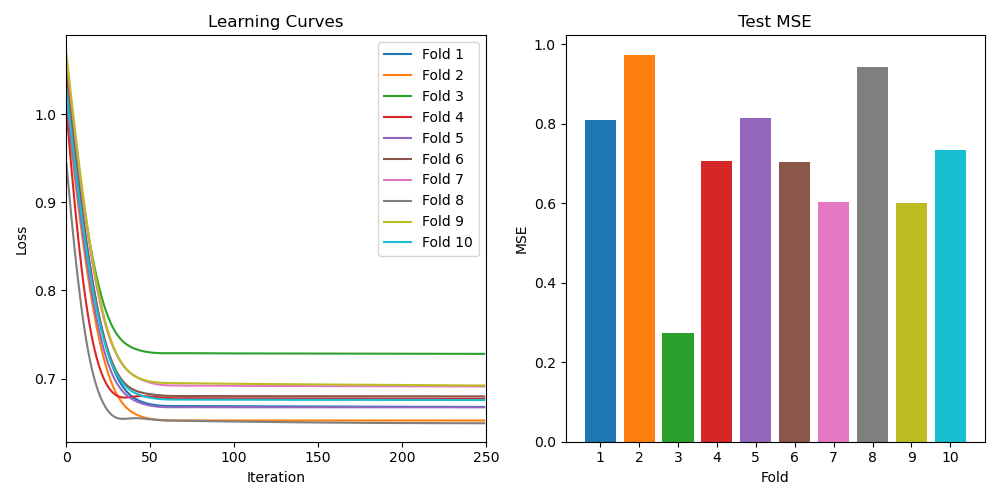
\includegraphics[width=0.8\textwidth]{./task_2/limited.png}
  \caption{Limited model's learnung curves}\label{fig:limited-curves}
\end{figure}
\begin{figure}[h!]
  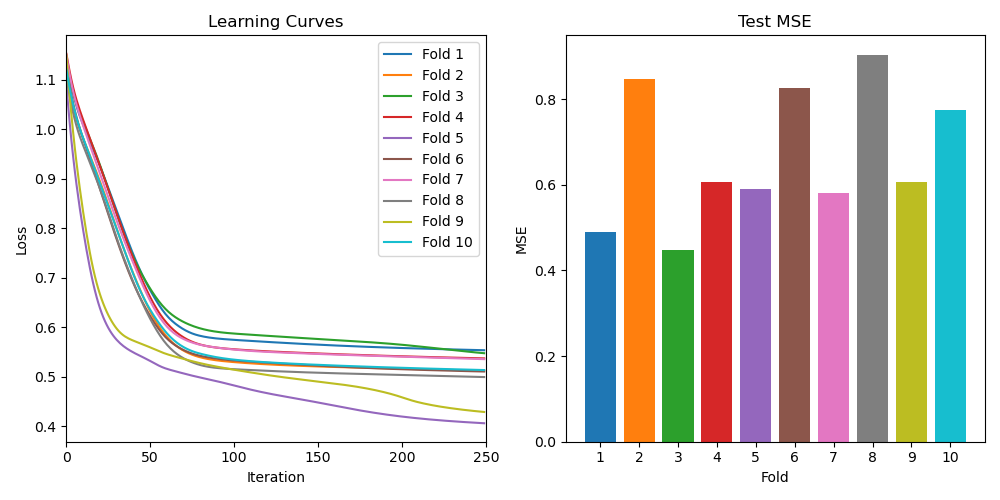
\includegraphics[width=0.8\textwidth]{./task_2/full_features.png}
  \caption{Full model's learnung curves}\label{fig:full-curves}
\end{figure}

\subsection{Boxplots}
\begin{figure}[h!]
  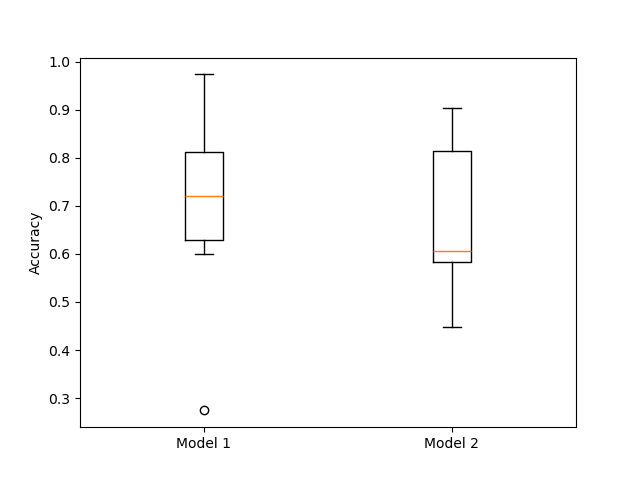
\includegraphics[width=0.8\textwidth]{./task_2/boxplot.png}
  \caption{Boxplots of both model's fold scores}\label{fig:boxplots}
\end{figure}

% \newpage
% \printbibliography
\end{document}
